\documentclass{beamer}

\usepackage{listings}
\usepackage{color}
\usepackage{svg}

\definecolor{pblue}{rgb}{0.13,0.13,1}
\definecolor{pgreen}{rgb}{0,0.5,0}
\definecolor{pred}{rgb}{0.9,0,0}
\definecolor{pgrey}{rgb}{0.46,0.45,0.48}

\usepackage{listings}
\lstset{language=Java,
  showspaces=false,
  showtabs=false,
  breaklines=true,
  showstringspaces=false,
  breakatwhitespace=true,
  commentstyle=\color{pgreen},
  keywordstyle=\color{pblue},
  stringstyle=\color{pred},
  basicstyle=\ttfamily
}


\begin{document}
\title{Dependency injection}   
\author{Jonas Verhoelen} 
\date{\today} 

\frame{\titlepage} 

\frame{\frametitle{Table of contents}\tableofcontents} 

%% INTRODUCTION
\section{Introduction}
\frame{\frametitle{What you can expect}
\begin{itemize}
\item Minimal theory about Dependency injection and all connected topics
\item Examples to quickly understand the concepts
\item Tasks and exercises for the purpose of self-study
\end{itemize}
}

%% THEORY
\section{Theory} 
\frame{\frametitle{What is Dependency injection?}
\begin{itemize}
\item Design pattern and concept in Object oriented programming
\item Get rid of hard-coded dependencies and replace by loose coupling
\item Moves the resolution of dependencies from compile-time to runtime
\item Very practical to create extendable and maintainable software, especially in big projects
\item Part of a lot of Frameworks which take even more workload from you
\item ...something you \textbf{definitely have to} get familiar with!
\end{itemize}
}

%% EXAMPLE
\section{Example} 
\frame{\frametitle{Classic coupling (composition)}

\lstinputlisting[language=Java, firstline=1, lastline=20]{src/ServeOrderRunnable.java}
}

\frame{\frametitle{Classic coupling (aggregation) - explanation}

This was a minimal example for a simple aggregation between the classes ServeOrderRunnable and Restaurant. ServeOrderRunnable owns Restaurant but also other classes and objects can own it. The Restaurant is independent from ServeOrderRunnable and does not need it in order to be created or maintained.

\begin{center}
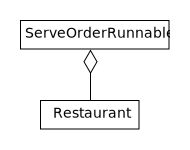
\includegraphics[scale=0.7]{img/aggregation.png}
\end{center}
}

\frame{\frametitle{Simplifying the situation - DI}
\lstinputlisting[language=Java, firstline=1, lastline=17]{src/ServeOrderRunnable_DI.java}
}

\frame{\frametitle{Simplifying the situation - DI2}

Huh? What happened?\\
We do not have to pass the Restaurant to the ServeOrderRunnable via the constructor anymore. The instance variable "restaurant" furthermore has a strange annotation above - @Autowired.\\
It's very simple: the annotation tells the framework (could be Java Spring in this example) that this instance variable should be injected from the available services.

So:
\begin{itemize}
\item The class Restaurant is a service
\item @Autowired marks that this instance variable should be initialized with an object of the class Restaurant
\item A framework or self-written facility maintains instances of services and can inject them

\end{itemize}
}

\frame{\frametitle{Conclusion from the example}

Dependency injection...

\begin{itemize}
\item makes dependencies the problems of someone different (be lazy!).
\item takes responsibilities from classes (one problem less).
\item transfers responsibility to create, maintain and inject dependencies to one central mechanism.
\item is handled by a lot of frameworks so you can just use it out of the box without caring.
\item also helps you testing, when complex dependencies are involved.
\end{itemize}
}


%\section{Abschnitt Nr. 2} 
%\subsection{Listen I}
%\frame{\frametitle{Aufz\"ahlung}
%\begin{itemize}
%\item Einf\"uhrungskurs in \LaTeX  
%\item Kurs 2  
%\item Seminararbeiten und Pr\"asentationen mit \LaTeX 
%\item Die Beamerclass 
%\end{itemize} 
%}
%
%\frame{\frametitle{Aufz\"ahlung mit Pausen}
%\begin{itemize}
%\item  Einf\"uhrungskurs in \LaTeX \pause 
%\item  Kurs 2 \pause 
%\item  Seminararbeiten und Pr\"asentationen mit \LaTeX \pause 
%\item  Die Beamerclass
%\end{itemize} 
%}
%
%\subsection{Listen II}
%\frame{\frametitle{Numerierte Liste}
%\begin{enumerate}
%\item  Einf\"uhrungskurs in \LaTeX 
%\item  Kurs 2
%\item  Seminararbeiten und Pr\"asentationen mit \LaTeX 
%\item  Die Beamerclass
%\end{enumerate}
%}
%\frame{\frametitle{Numerierte Liste mit Pausen}
%\begin{enumerate}
%\item  Einf\"uhrungskurs in \LaTeX \pause 
%\item  Kurs 2 \pause 
%\item  Seminararbeiten und Pr\"asentationen mit \LaTeX \pause 
%\item  Die Beamerclass
%\end{enumerate}
%}
%
%\section{Abschnitt Nr.3} 
%\subsection{Tabellen}
%\frame{\frametitle{Tabellen}
%\begin{tabular}{|c|c|c|}
%\hline
%\textbf{Zeitpunkt} & \textbf{Kursleiter} & \textbf{Titel} \\
%\hline
%WS 04/05 & Sascha Frank &  Erste Schritte mit \LaTeX  \\
%\hline
%SS 05 & Sascha Frank & \LaTeX \ Kursreihe \\
%\hline
%\end{tabular}}
%
%
%\frame{\frametitle{Tabellen mit Pause}
%\begin{tabular}{c c c}
%A & B & C \\ 
%\pause 
%1 & 2 & 3 \\  
%\pause 
%A & B & C \\ 
%\end{tabular} }
%
%
%\section{Abschnitt Nr. 4}
%\subsection{Bl\"ocke}
%\frame{\frametitle{Bl\"ocke}
%
%\begin{block}{Blocktitel}
%Blocktext 
%\end{block}
%
%\begin{exampleblock}{Blocktitel}
%Blocktext 
%\end{exampleblock}
%
%
%\begin{alertblock}{Blocktitel}
%Blocktext 
%\end{alertblock}
%}
\end{document}

